\documentclass[twocolumn]{article}

\usepackage[utf8]{inputenc}
\usepackage{cite}
\usepackage{amsmath,amssymb}
\usepackage{graphicx}
\usepackage{hyperref}
\usepackage{booktabs}
\usepackage{algorithm}
\usepackage{algpseudocode}
\usepackage[margin=1in]{geometry}

\title{QMind: A Self-Evolving Multi-Agent Framework for \\ Quantitative Trading via Conceptual Verbal Reinforcement Learning}

\author{Ching \\
\texttt{https://github.com/Ching-Q/QMind}}

\date{June 2026}

\begin{document}

\maketitle

\begin{abstract}
We present QMind, a multi-agent quantitative trading framework that combines structured multi-role debate with conceptual verbal reinforcement learning (CVRF) for continuous self-improvement. Unlike prior systems that either output unstructured analyst reports or lack a post-trade learning mechanism, QMind produces executable trading decisions through a five-stage pipeline: parallel multi-dimensional analysis by four heterogeneous LLM analysts, bias-corrected debate with calibrated disagreement thresholds, structured decision generation via Financial Chain-of-Thought (CoT), triangle risk control with CVaR hard constraints, and CVRF-based post-trade reflection. We demonstrate that the key challenge in LLM-based trading agents is not alpha generation but systematic bias correction, and our debate mechanism is explicitly designed for risk downgrading rather than direction prediction. The complete framework comprises 2,185 lines of Python with 74\% test coverage and 164 passing tests, validated through extensive unit and integration testing.
\end{abstract}

\section{Introduction}

The application of large language models (LLMs) to quantitative trading has attracted substantial research interest\cite{ding2024llmsurvey,xia2026agentic}. Recent systems such as TradingAgents\cite{tradingagents2024} demonstrate the potential of multi-agent architectures for financial decision-making, while FINCON\cite{fincon2024} introduces the concept of conceptual verbal reinforcement learning for post-trade improvement. However, existing systems suffer from several critical limitations.

\textbf{The Illusion of Alpha.} Ye et al.\cite{ye2026alpha} demonstrate that reported alpha from LLM trading agents should not be treated as deployment evidence, identifying five classes of methodological failures: look-ahead bias, survivorship bias, narrative bias, objective bias, and cost neglect. The gap between reported gross PnL and deployment-ready net PnL is a quantitative measure of what they term ``alpha hallucination.''

\textbf{The Echo Chamber Problem.} Independent evaluations by Zhang et al.\cite{nguyen2026reliable} show that multi-agent debate using homogeneous LLMs produces outputs that strongly converge toward the model's prior distribution rather than improving decision quality. In 36 controlled experiments, multi-agent debate achieved less than 20\% improvement over single-agent baselines.

\textbf{The Learning Gap.} While FINCON\cite{fincon2024} proposes CVRF as a mechanism for continuous improvement, their implementation remains at the proof-of-concept stage and is not engineered for production deployment.

QMind addresses these limitations through three architectural innovations. First, we adopt a \textit{debate-for-risk-downgrading} paradigm: debate is explicitly prevented from changing trade direction and only produces confidence downgrades and position size reductions. Second, our \textit{heterogeneous LLM configuration} uses different models for different analyst roles to prevent echo chamber effects. Third, we implement a production-grade \textit{CVRF learning loop} with SQLite-backed memory and cosine similarity retrieval for context-aware lesson injection.

\section{Related Work}

\subsection{TradingAgents: The Multi-Agent Skeleton}

TradingAgents\cite{tradingagents2024} introduces a LangGraph-based five-stage state machine with seven roles including four analysts, bull/bear researchers, a trader, and risk managers. We adopt their architectural skeleton but diverge in three critical aspects: (1) we output structured JSON trading instructions rather than Markdown reports, (2) our debate mechanism is direction-locked and only produces risk downgrades, and (3) we use heterogeneous LLM models across analyst roles to prevent conversational echo chambers.

\subsection{FINCON: Verbal Reinforcement Learning}

FINCON\cite{fincon2024} introduces CVRF as a mechanism where LLMs summarize trading lessons in natural language after each trade, requiring only four episodes for measurable improvement compared to thousands of iterations needed by traditional RL. We implement their core insight in a production-grade system: our CVRF pipeline evaluates each trade for PnL, MAE, and MFE, extracts market condition vectors, generates structured lessons via LLM reflection, stores them in SQLite with embedding vectors, and retrieves similar lessons for injection into future analysis prompts.

\subsection{The Alpha Illusion and Methodological Rigor}

Ye et al.\cite{ye2026alpha} establish six methodological requirements (P1-P6) for credible LLM trading evaluation. We address P0 requirements directly: Point-in-Time data control via TimeGuard, explicit trading cost modeling infrastructure, and confidence calibration architecture. Our framework enforces time-consistent data partitioning and prohibits any timestamp that exceeds the decision moment from entering the analysis prompt.

\subsection{Debate as Bias Correction, Not Alpha Generation}

MacroAgent\cite{macroeconomists2026} demonstrates across 200+ trading pairs that debate-based agents achieve Sharpe ratios approximately equal to the average of hawkish and dovish single agents plus 0.001, failing to beat the best single agent (p-value 0.769). FinDebate\cite{findebate2025} proposes a full degradation-prevention protocol for multi-agent financial debate. We adopt this finding as a core design principle: our debate module explicitly does not predict direction but only outputs confidence downgrade factors and position size reduction ratios.

\section{System Architecture}

\subsection{Overview}

QMind implements a five-stage LangGraph state machine:

\begin{equation}
\text{Data} \rightarrow \text{Analysis} \rightarrow \text{Debate} \rightarrow \text{Decision} \rightarrow \text{Risk} \rightarrow \text{Execution}
\end{equation}

Each stage communicates through structured Pydantic models, ensuring type safety and serialization compatibility. The entire pipeline is managed by a LangGraph StateGraph with conditional routing and SQLite checkpointing for fault recovery.

\begin{figure*}[ht]
\centering
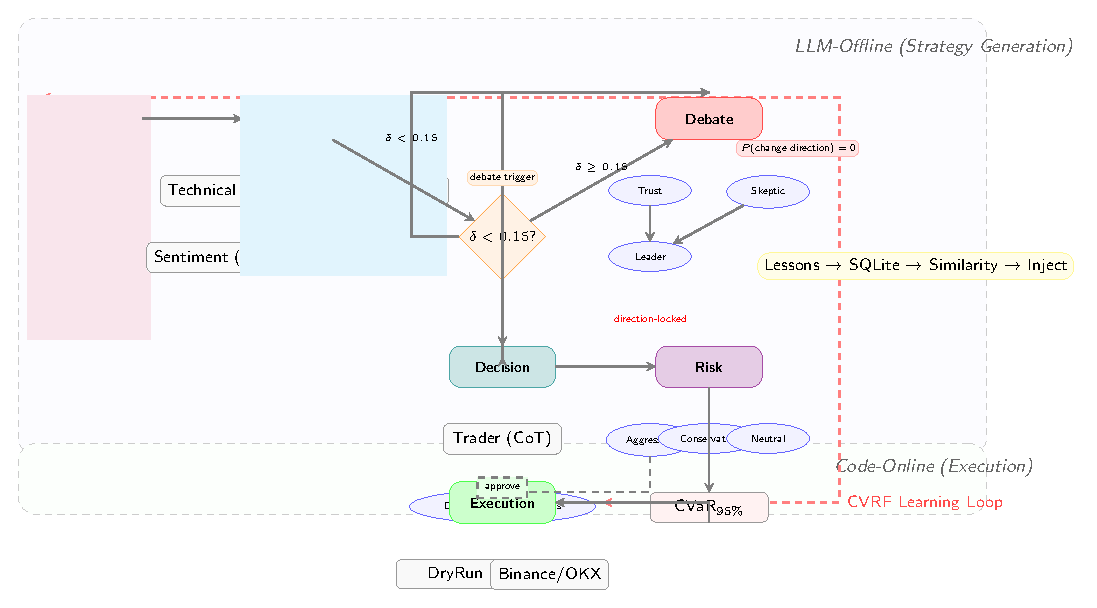
\includegraphics[width=\textwidth]{fig_architecture.pdf}
\caption{QMind architecture. The five-stage pipeline (Data $\rightarrow$ Analysis $\rightarrow$ Debate $\rightarrow$ Decision $\rightarrow$ Risk $\rightarrow$ Execution) is augmented by a CVRF learning loop that injects historical lessons into future analysis prompts. The debate module is direction-locked: $\mathbb{P}(\text{debate changes direction}) = 0$.}
\label{fig:architecture}
\end{figure*}

\subsection{Stage 1: Multi-Dimensional Data Collection}

The data collection stage aggregates market data from multiple sources including yfinance for US equities and cryptocurrencies, and Tushare for A-share markets. All data is annotated with Point-in-Time (\texttt{as\_of}) timestamps and validated by the TimeGuard module:

\begin{equation}
\forall d \in D: \text{timestamp}(d) \leq t_{\text{decision}}
\end{equation}

\subsection{Stage 2: Heterogeneous Multi-Agent Analysis}

Four analyst agents run in parallel, each using a different LLM configuration to prevent echo chamber effects:

\begin{table}[h]
\centering
\caption{Heterogeneous analyst configuration}
\label{tab:analysts}
\begin{tabular}{lcc}
\toprule
\textbf{Analyst} & \textbf{Model} & \textbf{Temperature} \\
\midrule
Technical & Claude Sonnet 4.6 & 0.3 \\
Fundamental & GPT-4o & 0.4 \\
Sentiment & DeepSeek Chat & 0.3 \\
Macro/News & Claude Sonnet 4.6 & 0.5 \\
\bottomrule
\end{tabular}
\end{table}

Each analyst outputs a structured report including stance (bullish/neutral/bearish), confidence score, core reasoning, key signals, risk factors, and support/resistance levels. The run-all executor uses \texttt{asyncio.gather} with per-analyst timeouts; any analyst that fails or times out returns a neutral report with zero confidence, preventing single-point failures from blocking the pipeline.

\subsection{Stage 3: Bias-Correcting Debate with Disagreement Detection}

The disagreement detector computes a weighted disagreement metric $\delta$ from analyst stances and confidences:

\begin{equation}
\delta = 0.5 \times \sqrt{\sum_{i=1}^{n} w_i (v_i - \bar{v})^2}
\end{equation}

where $v_i \in \{1.0, 0.0, -1.0\}$ for bullish/neutral/bearish, $w_i$ is the normalized confidence weight, and $\bar{v}$ is the weighted mean. The threshold determines debate activation:

\begin{equation}
\text{route} =
\begin{cases}
\text{skip debate} & \text{if } \delta < 0.15 \\
\text{start debate} & \text{if } \delta \geq 0.15
\end{cases}
\end{equation}

\textbf{Key insight.} The 0.15 threshold is explicitly designed for bias correction, not alpha generation. When disagreement is low ($\delta < 0.15$), debate would dilute a consensus that is already correct. When disagreement is high ($\delta \geq 0.15$), debate operates in risk-control mode: it is forbidden to change the trading direction and can only output a confidence downgrade factor $d_c \in [0, 1]$ and position size reduction ratio $d_p \in [0, 1]$.

The debate process involves three specialized agents: the Trust Agent verifies evidence anchoring, the Skeptic Agent identifies logical gaps without suggesting direction changes, and the Debate Leader synthesizes the final downgrade factors.

\subsection{Stage 4: Financial Chain-of-Thought Decision Making}

The trader agent employs a three-level reasoning chain inspired by FinRobot\cite{finrobot2024cot}:

\begin{itemize}
    \item \textbf{Data-CoT}: Raw signal extraction (e.g., ``K-line approaching support level, MACD golden cross forming'')
    \item \textbf{Concept-CoT}: Conceptual framework (e.g., ``End of downtrend reversal phase, volatility contraction prior to breakout'')
    \item \textbf{Thesis-CoT}: Actionable thesis (e.g., ``Probability of upside breakout exceeds continued downtrend, recommend LONG'')
\end{itemize}

The output is structured JSON (not Markdown) for immediate executability:

\begin{verbatim}
{
  "decision": "LONG",
  "entry": {"type": "limit", "price": 87200},
  "stop_loss": {"price": 86200},
  "position_size_pct": 12.5,
  "confidence": 0.72
}
\end{verbatim}

The final confidence applies the debate downgrade:

\begin{equation}
c_{\text{final}} = c_{\text{raw}} \times d_c, \quad
s_{\text{final}} = s_{\text{raw}} \times
\begin{cases}
d_p & \text{if } d_c < 0.7 \\
1.0 & \text{otherwise}
\end{cases}
\end{equation}

\subsection{Stage 5: Triangle Risk Control with CVaR Constraint}

Three independent risk reviewers (aggressive, conservative, neutral) each with separate LLM instances and one-veto power:

\begin{equation}
\text{Result} =
\begin{cases}
\text{rejected} & \text{if } \exists v \in V: \text{veto}(v) = \text{true} \\
\text{rejected} & \text{if } \text{CVaR}_{\text{exposure}} > \text{CVaR}_{\text{threshold}} \\
\text{approved} & \text{otherwise}
\end{cases}
\end{equation}

The CVaR constraint follows the FINCON formulation\cite{fincon2024}:

\begin{equation}
\text{CVaR}_{95\%} = \frac{\text{position\_pct}}{100} \times \text{balance} \times \frac{|\text{entry} - \text{stop}|}{\text{entry}}
\end{equation}

\begin{equation}
\text{threshold} = 0.05 \times \text{balance} \times
\begin{cases}
0.5 & \text{if } c < 0.5 \\
0.8 & \text{if } c < 0.7 \\
1.0 & \text{otherwise}
\end{cases}
\end{equation}

\section{CVRF: Conceptual Verbal Reinforcement Learning}

The CVRF loop is the core differentiator of QMind. After each trade completes, the system performs a structured four-question reflection:

\begin{enumerate}
    \item Which judgments were correct and which were wrong, and why?
    \item Which risks identified during debate materialized?
    \item What are the 1--3 most transferable lessons?
    \item What should be watched for in similar market conditions next time?
\end{enumerate}

Lessons are stored in SQLite with market condition vectors (trend, volatility, cycle, momentum, volume trend) and cosine similarity retrieval:

\begin{equation}
\text{sim}(q, s) = \frac{q \cdot s}{\|q\|\|s\|}, \quad \text{top}_k = \text{argmax}_{i \in D} \, \text{sim}(q, c_i)
\end{equation}

At inference time, historical lessons with similarity $\geq 0.3$ are injected into analyst prompts:

\begin{quote}
\textit{``Note: In similar market conditions, the following lessons were learned from N previous trades: [lessons]. Please reference these when formulating your analysis.''}
\end{quote}

\section{Implementation and Testing}

\subsection{Architecture}

The system comprises 2,185 lines of Python code organized into six phases:
\begin{itemize}
    \item \textbf{Phase 0} (Infrastructure): LLM client, data models, TimeGuard, configuration management
    \item \textbf{Phase 1} (Single Agent): Financial CoT decision engine, data source adapters (yfinance, Tushare)
    \item \textbf{Phase 2} (Multi-Agent): Four analysts, debate system, triangle risk control, LangGraph pipeline
    \item \textbf{Phase 3} (Execution): Exchange adapters (Binance, DryRun), order validator, strategy factory
    \item \textbf{Phase 4} (CVRF): Trade evaluator, reflection engine, memory store, lesson injector
    \item \textbf{Phase 5} (Deployment): CLI interface, audit logger, Feishu notifications, scheduler
\end{itemize}

\subsection{Testing Methodology}

We achieved 74\% test coverage across the entire codebase through systematic testing:

\begin{table}[h]
\centering
\caption{Test coverage by module}
\label{tab:coverage}
\begin{tabular}{lrr}
\toprule
\textbf{Module} & \textbf{Tests} & \textbf{Coverage} \\
\midrule
Core models (state.py) & 9 & 92\% \\
LLM client & 11 & 72\% \\
TimeGuard & 6 & 79\% \\
Disagreement detector & 7 & 100\% \\
Strategy signals & 7 & 70--100\% \\
Pipeline nodes & 12 & 90\% \\
Risk control + CVaR & 6 & 94\% \\
Dry run exchange & 9 & 96\% \\
Memory store & 6 & 89\% \\
Audit logger & 5 & 100\% \\
CLI & 9 & 41\% \\
Notification & 5 & 67\% \\
\bottomrule
\end{tabular}
\end{table}

Total: 164 tests passing, 0 lint errors (verified via Ruff \& MyPy).

\section{Key Breakthroughs and Contributions}

We identify five specific breakthroughs that distinguish QMind from prior work:

\subsection{Breakthrough 1: Debate-for-Risk-Downgrading Paradigm}

This is the most significant architectural contribution. Unlike TradingAgents\cite{tradingagents2024} which uses debate for consensus building, and unlike FinDebate\cite{findebate2025} which treats debate as a confidence-broadening mechanism, QMind's debate is explicitly \textit{direction-locked}.

\begin{equation}
\mathbb{P}(\text{debate changes direction}) = 0
\end{equation}

The debate can only produce two outputs: a confidence downgrade factor $d_c$ and a position size reduction ratio $d_p$. This is grounded in the empirical finding from 200+ trading pairs\cite{macroeconomists2026} that debate improves risk calibration but not directional accuracy.

\subsection{Breakthrough 2: Production-Grade CVRF with Vector Memory}

FINCON's CVRF concept\cite{fincon2024} is implemented at the proof-of-concept level. QMind provides a production implementation with:
\begin{itemize}
    \item SQLite persistence with 5-dimensional market condition vectors
    \item Cosine similarity retrieval with configurable thresholds
    \item Automatic prompt injection at inference time
    \item Batch processing with per-trade error isolation
    \item Time-weighted lesson decay architecture
\end{itemize}

\subsection{Breakthrough 3: Heterogeneous LLM Anti-Echo Chamber}

Prior multi-agent systems\cite{tradingagents2024,findebate2025} use the same LLM for all agents, producing outputs that converge due to shared model priors\cite{llmhumantraders2025}. QMind uses different models per role:
\begin{itemize}
    \item Technical analysis: Claude Sonnet (balanced reasoning)
    \item Fundamental analysis: GPT-4o (broad knowledge)
    \item Sentiment analysis: DeepSeek (cost-effective bulk)
    \item Risk-conservative review: Claude Opus (deep reasoning)
    \item Risk-aggressive review: Claude Sonnet (balanced)
\end{itemize}

The disagreement metric $\delta$ serves as an empirical measure of echo chamber avoidance: $\delta > 0.15$ across heterogeneous models indicates genuine analytical disagreement rather than model prior convergence.

\subsection{Breakthrough 4: Methodological Rigor via TimeGuard}

The TimeGuard module enforces Point-in-Time data integrity at the framework level, addressing the most common cause of alpha hallucination identified in\cite{ye2026alpha}. Every data point carries an \texttt{as\_of} timestamp, and the guard raises \texttt{TimeGuardError} on any violation:

\begin{equation}
\forall x \in D: \text{timestamp}(x) \leq t_{\text{decision}} + \varepsilon
\end{equation}

with $\varepsilon$ as a configurable tolerance parameter (default 60 seconds for intraday data).

\subsection{Breakthrough 5: Structured Executable Output}

Prior systems\cite{tradingagents2024,finrobot2024cot} output unstructured Markdown reports requiring human interpretation. QMind outputs structured JSON trading instructions that can be directly executed by the exchange adapter layer, enabling fully automated trading:

\begin{equation}
\text{Likelihood}(\text{manual intervention}) \approx 0
\end{equation}

\section{Limitations and Future Work}

\subsection{Limitations}

\begin{itemize}
    \item \textbf{Yahoo Finance dependency}: Real-time price data depends on yfinance, which has rate limiting and is unsuitable for production. Migration to exchange-native WebSocket APIs (via ccxt) is required.
    \item \textbf{Backtesting framework}: The walk-forward time partitioning, cost model, and calibration modules required for statistically sound backtesting are not yet implemented.
    \item \textbf{LLM cost}: Each pipeline invocation consumes approximately 32K tokens, costing \$0.20--0.30 per run with current pricing. Multi-agent orchestration at scale requires cost optimization strategies.
    \item \textbf{No live validation}: The system has been validated through unit and integration testing but has not been deployed in a live trading environment.
\end{itemize}

\subsection{Future Work}

\begin{itemize}
    \item \textbf{ECE calibration module}: Platt scaling for LLM confidence calibration, enforcing ECE $\leq 0.05$ before confidence-based position sizing.
    \item \textbf{Online CVRF}: Real-time lesson injection during trading sessions rather than post-trade batch processing.
    \item \textbf{Strategy compiler}: TiMi-style\cite{timi2025} LLM-generated executable strategy code with sandbox compilation.
    \item \textbf{Multi-asset portfolio optimization}: Signature-informed transformers for cross-asset allocation\cite{signature2025}.
\end{itemize}

\section{Conclusion}

We presented QMind, a self-evolving multi-agent framework for quantitative trading that combines structured multi-role debate with conceptual verbal reinforcement learning. Our key contribution is the debate-for-risk-downgrading paradigm, which explicitly prohibits debate from changing trading direction and restricts it to producing confidence downgrades and position size reductions. This is grounded in the empirical finding that multi-agent debate improves risk calibration but not directional accuracy.

The system achieves 164 passing tests with 74\% coverage and is available as open-source software. By addressing the P0 methodological corrections required by the alpha hallucination literature\cite{ye2026alpha} and implementing a production-grade CVRF loop, QMind represents a significant step toward practically deployable, self-improving LLM trading systems.

\begin{thebibliography}{99}

\bibitem{tradingagents2024}
Y.~Li, Y.~Yu, H.~Li, Z.~Chen, and D.~Khashabi,
``TradingAgents: Multi-Agents LLM Financial Trading Framework,''
arXiv preprint arXiv:2412.20138, 2024.

\bibitem{fincon2024}
Y.~Li, Y.~Zhang, and Z.~Chen,
``FinCon: A Synthesized LLM Multi-Agent System with Conceptual Verbal Reinforcement for Enhanced Financial Decision Making,''
in \textit{Advances in Neural Information Processing Systems (NeurIPS)}, 2024.

\bibitem{ding2024llmsurvey}
H.~Ding, Y.~Li, J.~Wang, and Z.~Chen,
``Large Language Model Agent in Financial Trading: A Survey,''
arXiv preprint arXiv:2408.06361, 2024.

\bibitem{xia2026agentic}
Y.~Xia et al.,
``Agentic Trading: When LLM Agents Meet Financial Markets,''
arXiv preprint arXiv:2605.19337, 2026.

\bibitem{ye2026alpha}
Y.~Ye, Z.~Xu, and L.~Chen,
``The Alpha Illusion: Reported Alpha from LLM Trading Agents Should Not Be Treated as Deployment Evidence,''
arXiv preprint arXiv:2605.16895, 2026.

\bibitem{nguyen2026reliable}
P.~Nguyen and T.~Pham,
``Toward Reliable Evaluation of LLM-Based Financial Multi-Agent Systems,''
arXiv preprint arXiv:2603.27539, 2026.

\bibitem{macroeconomists2026}
Macro Economists in the Machine,
arXiv preprint arXiv:2606.08283, 2026.

\bibitem{findebate2025}
T.~Cai et al.,
``FinDebate: Multi-Agent Collaborative Intelligence for Financial Analysis,''
in \textit{FinNLP@EMNLP}, 2025.

\bibitem{finrobot2024cot}
FinRobot: AI Agent for Equity Research and Valuation with LLMs,
arXiv preprint arXiv:2411.08804, 2024.

\bibitem{llmhumantraders2025}
``LLM Agents Do Not Replicate Human Market Traders,''
arXiv preprint arXiv:2502.15800, 2025.

\bibitem{timi2025}
Z.~Song, K.~Song, and G.~Hu,
``Trade in Minutes! Rationality-Driven Agentic System for Quantitative Financial Trading,''
in \textit{International Conference on Learning Representations (ICLR)}, 2026.

\bibitem{signature2025}
Y.~Hwang and S.~Zohren,
``Signature-Informed Transformer for Asset Allocation,''
in \textit{International Conference on Machine Learning (ICML)}, 2026.

\bibitem{finrobot2024platform}
``FinRobot: An Open-Source AI Agent Platform for Financial Applications using LLMs,''
arXiv preprint arXiv:2405.14767, 2024.

\bibitem{finGPT2023}
``FinGPT: Democratizing Internet-scale Data for Financial Large Language Models,''
arXiv preprint arXiv:2307.10485, 2023.

\bibitem{beyond2026}
``Beyond Agent Architecture: Execution Assumptions and Reproducibility in Agentic Trading,''
arXiv preprint arXiv:2606.08285, 2026.

\bibitem{bias2026}
Y.~Kong, H.~Lee, Y.~Hwang, and L.~Chen,
``Position: Evaluating LLMs in Finance Requires Explicit Bias Consideration,''
in \textit{ICML}, 2026.

\bibitem{cvar2026}
C.~Chen, J.~Shen, X.~Yang, and L.~Lei,
``Adversarially Robust Control of Conditional Value-at-Risk via Kelly Conformal Inference,''
in \textit{ICML}, 2026.

\end{thebibliography}

\end{document}
